\subsection{DK-Kogebogen}
\label{subsec:dk-kogebogen}

DK-Kogebogen er en webapplikation, som tilbyder en lang række funktioner, hvoraf ``tøm køleskabet'' er en af dem. Udover ``tøm køleskabet'', tilbyder DK-kogebogen også en ugentlig madplan, et kæmpe opskriftsregister, en ekstern hjemmeside med fokus på viden omkring mad (energiindhold, vitaminindhold osv.) og en kalorieberegner. Siden har et omfang på over 36.000 opskrifter, hvilket er det klart største antal blandt de undersøgte systemer. De mange opskrifter er indsendt og lavet af brugere af hjemmesiden. Dette er både positivt og negativt. Der kan forekomme en del fejl i opskrifterne hvis de ikke først bliver gennemrettet. DK-Kogebogen skriver på deres hjemmeside, om de indsendte opskrifter:

%kilde: http://dk-kogebogen.dk/opskrifts-service/indsend-opskrift.php
\begin{quote}
``Opskriften kan ses med det samme, men der vil senere blive rettet lidt til i teksterne.'' \cite{dk-kog-indtastopskrift}
\end{quote}

Det er altså muligt for alle at indsende opskrifter, som er fulde af fejl, og disse vil alligevel være synlige på siden. Til gengæld skaber det mulighed for, at den enkelte bruger føler sig mere knyttet til siden, da han/hun har et personligt engagement i den, fordi de indsender deres egne opskrifter; og dette vil resultere i en overordnet højere brugeraktivitet. Det skal noteres, at de 36.000 opskrifter ikke er unikke. Det vil sige, at der godt kan eksistere flere forskellige varianter af den samme opskrift; \fx er der 17 forskellige varianter af Boller i Karry, hvilket kan virke uoverskueligt.

``Tøm køleskabs''-funktionen er placeret i toppen af DK-Kogebogens forside og er vist i \figref{fig:dk-kogebogen1}. Her kan brugeren indtaste så mange ingredienser der er brug for, inden for en grænse på 55 karakter. For at systemet kan identificere ingredienser, skal der mellem hver ingrediens, som brugeren indtaster, være et mellemrumstegn. Begrænsningen på 55 tegn betyder, at der maksimalt kan søges på ca. 8-10 ingredienser af gangen (forudsat at ingrediensnavne er 5-7 bogstaver lange).

\begin{figure}[H]
\centering
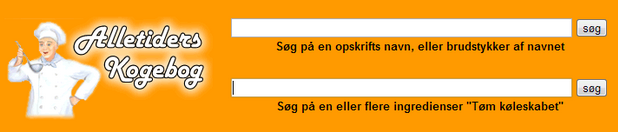
\includegraphics[scale=0.7]{billeder/forbilleder/dk-kogebogen.png}
\capt{DK-Kogebogens ``Tøm køleskabet''-funktion. Funktionen er tilgængelig i toppen af forsiden, og enhver anden underside.}
\label{fig:dk-kogebogen1}
\end{figure}

Efter brugeren har søgt på opskrifter med en eller flere specifikke ingredienser, viser DK-Kogebogen en liste med alle de opskrifter, som indeholder ingredienserne. På \figref{fig:dk-kogebogen2} ses en del af den liste, som er resultatet ved søgning på ``Tomat Paprika Kartoffel''. Ud fra opskrifterne kan der findes et kamera-symbol og/eller et dokument-symbol, som respektivt fortæller brugeren, om der er et billede af den pågældende opskrift, og/eller at opskriftens næringsindhold er beregnet og vist. Brugeren vælger derefter en af opskrifterne han/hun finder mest interessant. 

\begin{figure}[H]
\centering
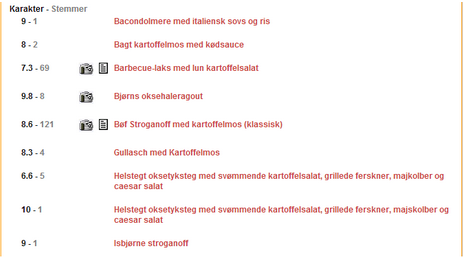
\includegraphics[scale=0.7]{billeder/forbilleder/dk-kogebogen2.png}
\capt{Liste af opskrifter, som indeholder ingredienserne Tomat, Paprika og Kartoffel.}
\label{fig:dk-kogebogen2}
\end{figure}

Inde på opskriftsvisningsiden er det i nogle tilfælde muligt at op- eller nedskalere portionsstørrelsen, mens der i andre tilfælde skaleres på antal personer. Derudover er der også nogle opskrifter, hvor det slet ikke er muligt at skalere. Her er brugeren i stedet for tvunget til selv at finde ud af, hvor stor en portion opskriften ca. passer til. Der er altså ikke overensstemmelse med, hvad portionerne skal angives i. Denne mangel på konsistens er endnu en af problematikkerne ved, at det er brugerne selv, som indsender opskrifterne. En endelig vurdering af DK-Kogebogen, findes i \secref{subsec:eksisterende.sammendrag}.
